% % Full page illustration
% \begin{figure}[!hbtp]
%     \centering
%     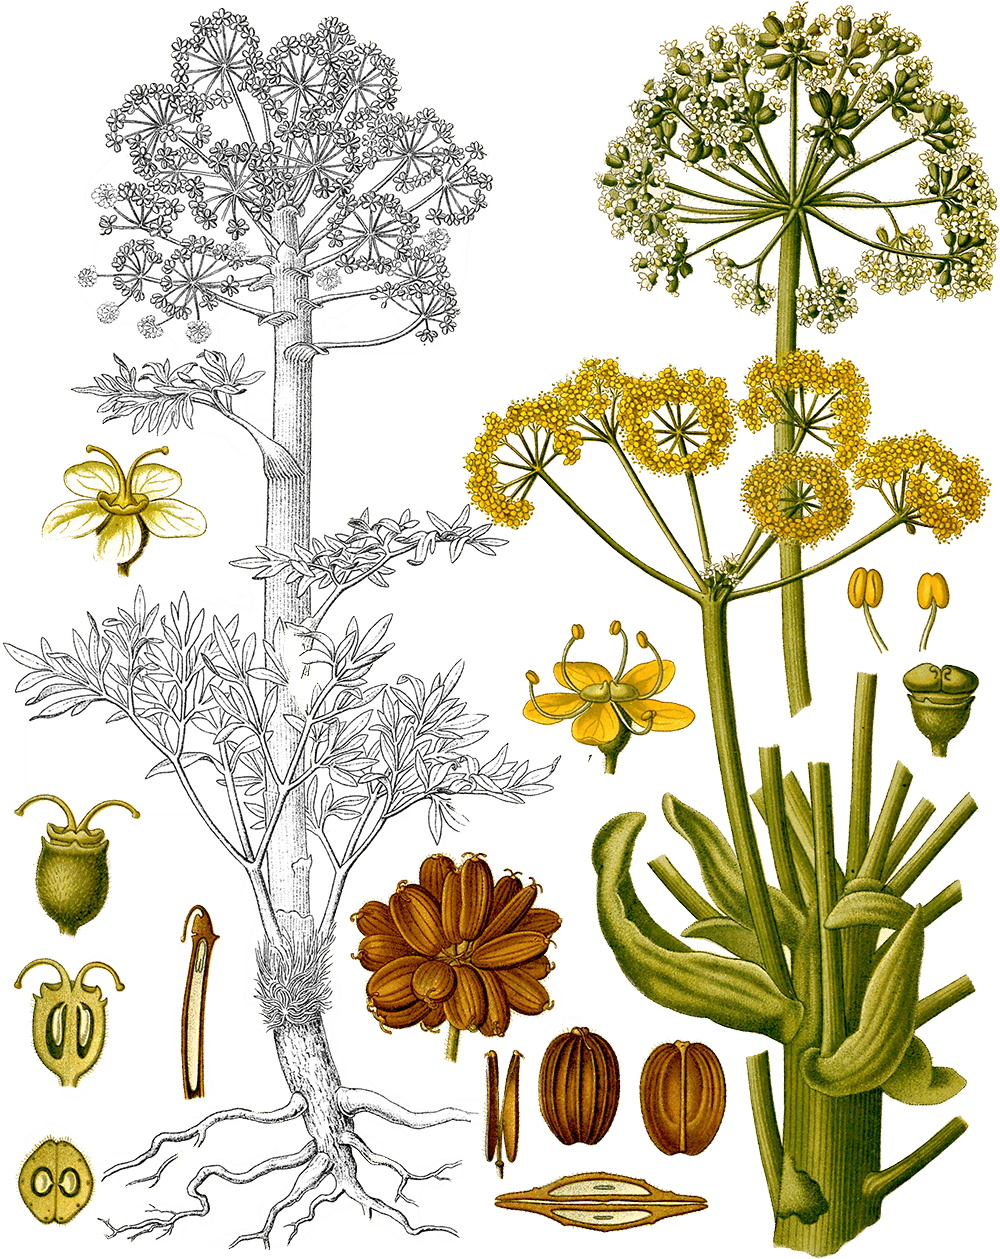
\includegraphics[width=\textwidth]{imgs/kohler/asafoetida_kohler_min.png}
%     \caption{\taxonn{Ferula foetida}{(Bunge) Regel} (syn. \taxonn{Ferula scorodosma}{Benth. \& Hook.}), one of the sources of asafoetida in Köhler's Medicinal Plants \pvolcite[]{2}[147]{kohler_kohlers_1887}.}
%     \label{fig:kohler_asafoetida}
% \end{figure}



\section{Asafoetida}
\label{sec:asafoetida}

\begin{spice}\label{spice:asafoetida}
\textsc{Asafoetida} \hfill \href{https://powo.science.kew.org/taxon/842277-1}{POWO} \\
\textbf{English:} \textit{asafoetida}; \textit{hing; devil's dung}. 
\textbf{Arabic:} {\arabicfont{حلتیت}} \textit{ḥiltīt}. 
\textbf{Chinese:} {\tradchinesefont{阿魏}} \textit{āwèi}. 
\textbf{Hungarian:} \textit{ördöggyökér} [devil's root]; \textit{aszatgyanta} [asat resin]; \textit{bűzös aszat} [stinking asat].  \\
\noindent{\color{black}\rule[0.5ex]{\linewidth}{.5pt}}
\begin{tabular}{@{}p{0.25\linewidth}@{}p{0.75\linewidth}@{}}
Plant species: & \taxonn{Ferula foetida}{(Bunge) Regel}; \textit{\taxonn{Ferula assa-foetida}{L.}; \textit{Ferula narthex}; et al.} \\
Family: & \textit{Apiaceae} \\
part used: & gum-resin (latex) \\
Region of origin: & Iran; W. and C. Asia \\
Cultivated in: & Iran; Afghanistan \\
Color: & from pale yellow to brown \\
\end{tabular}
\end{spice}

\begin{figure}[!ht]
	\vspace{-4ex}
	\centering
	\subfloat[\centering gum-resin ]{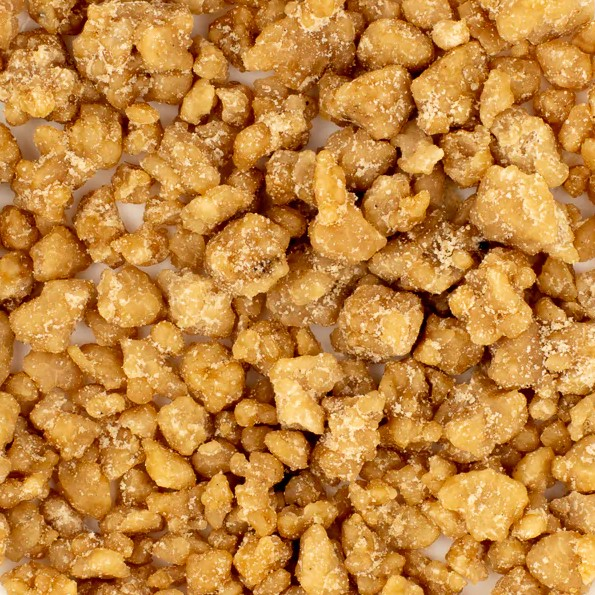
\includegraphics[width=0.3\linewidth]{imgs/spices/asafoetida-1.jpg}}
	\hfill
	\subfloat[\centering powder, colored with turmeric]{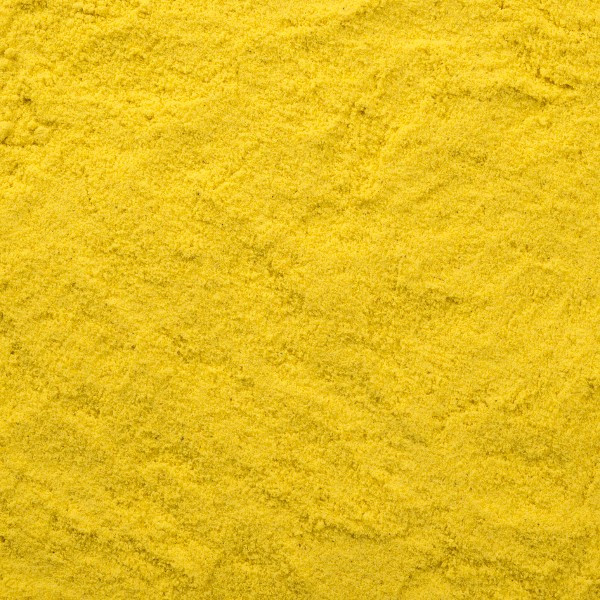
\includegraphics[width=0.3\linewidth]{imgs/spices/asafoetida-2.jpg}}
	\hfill
	\subfloat[\centering plant]{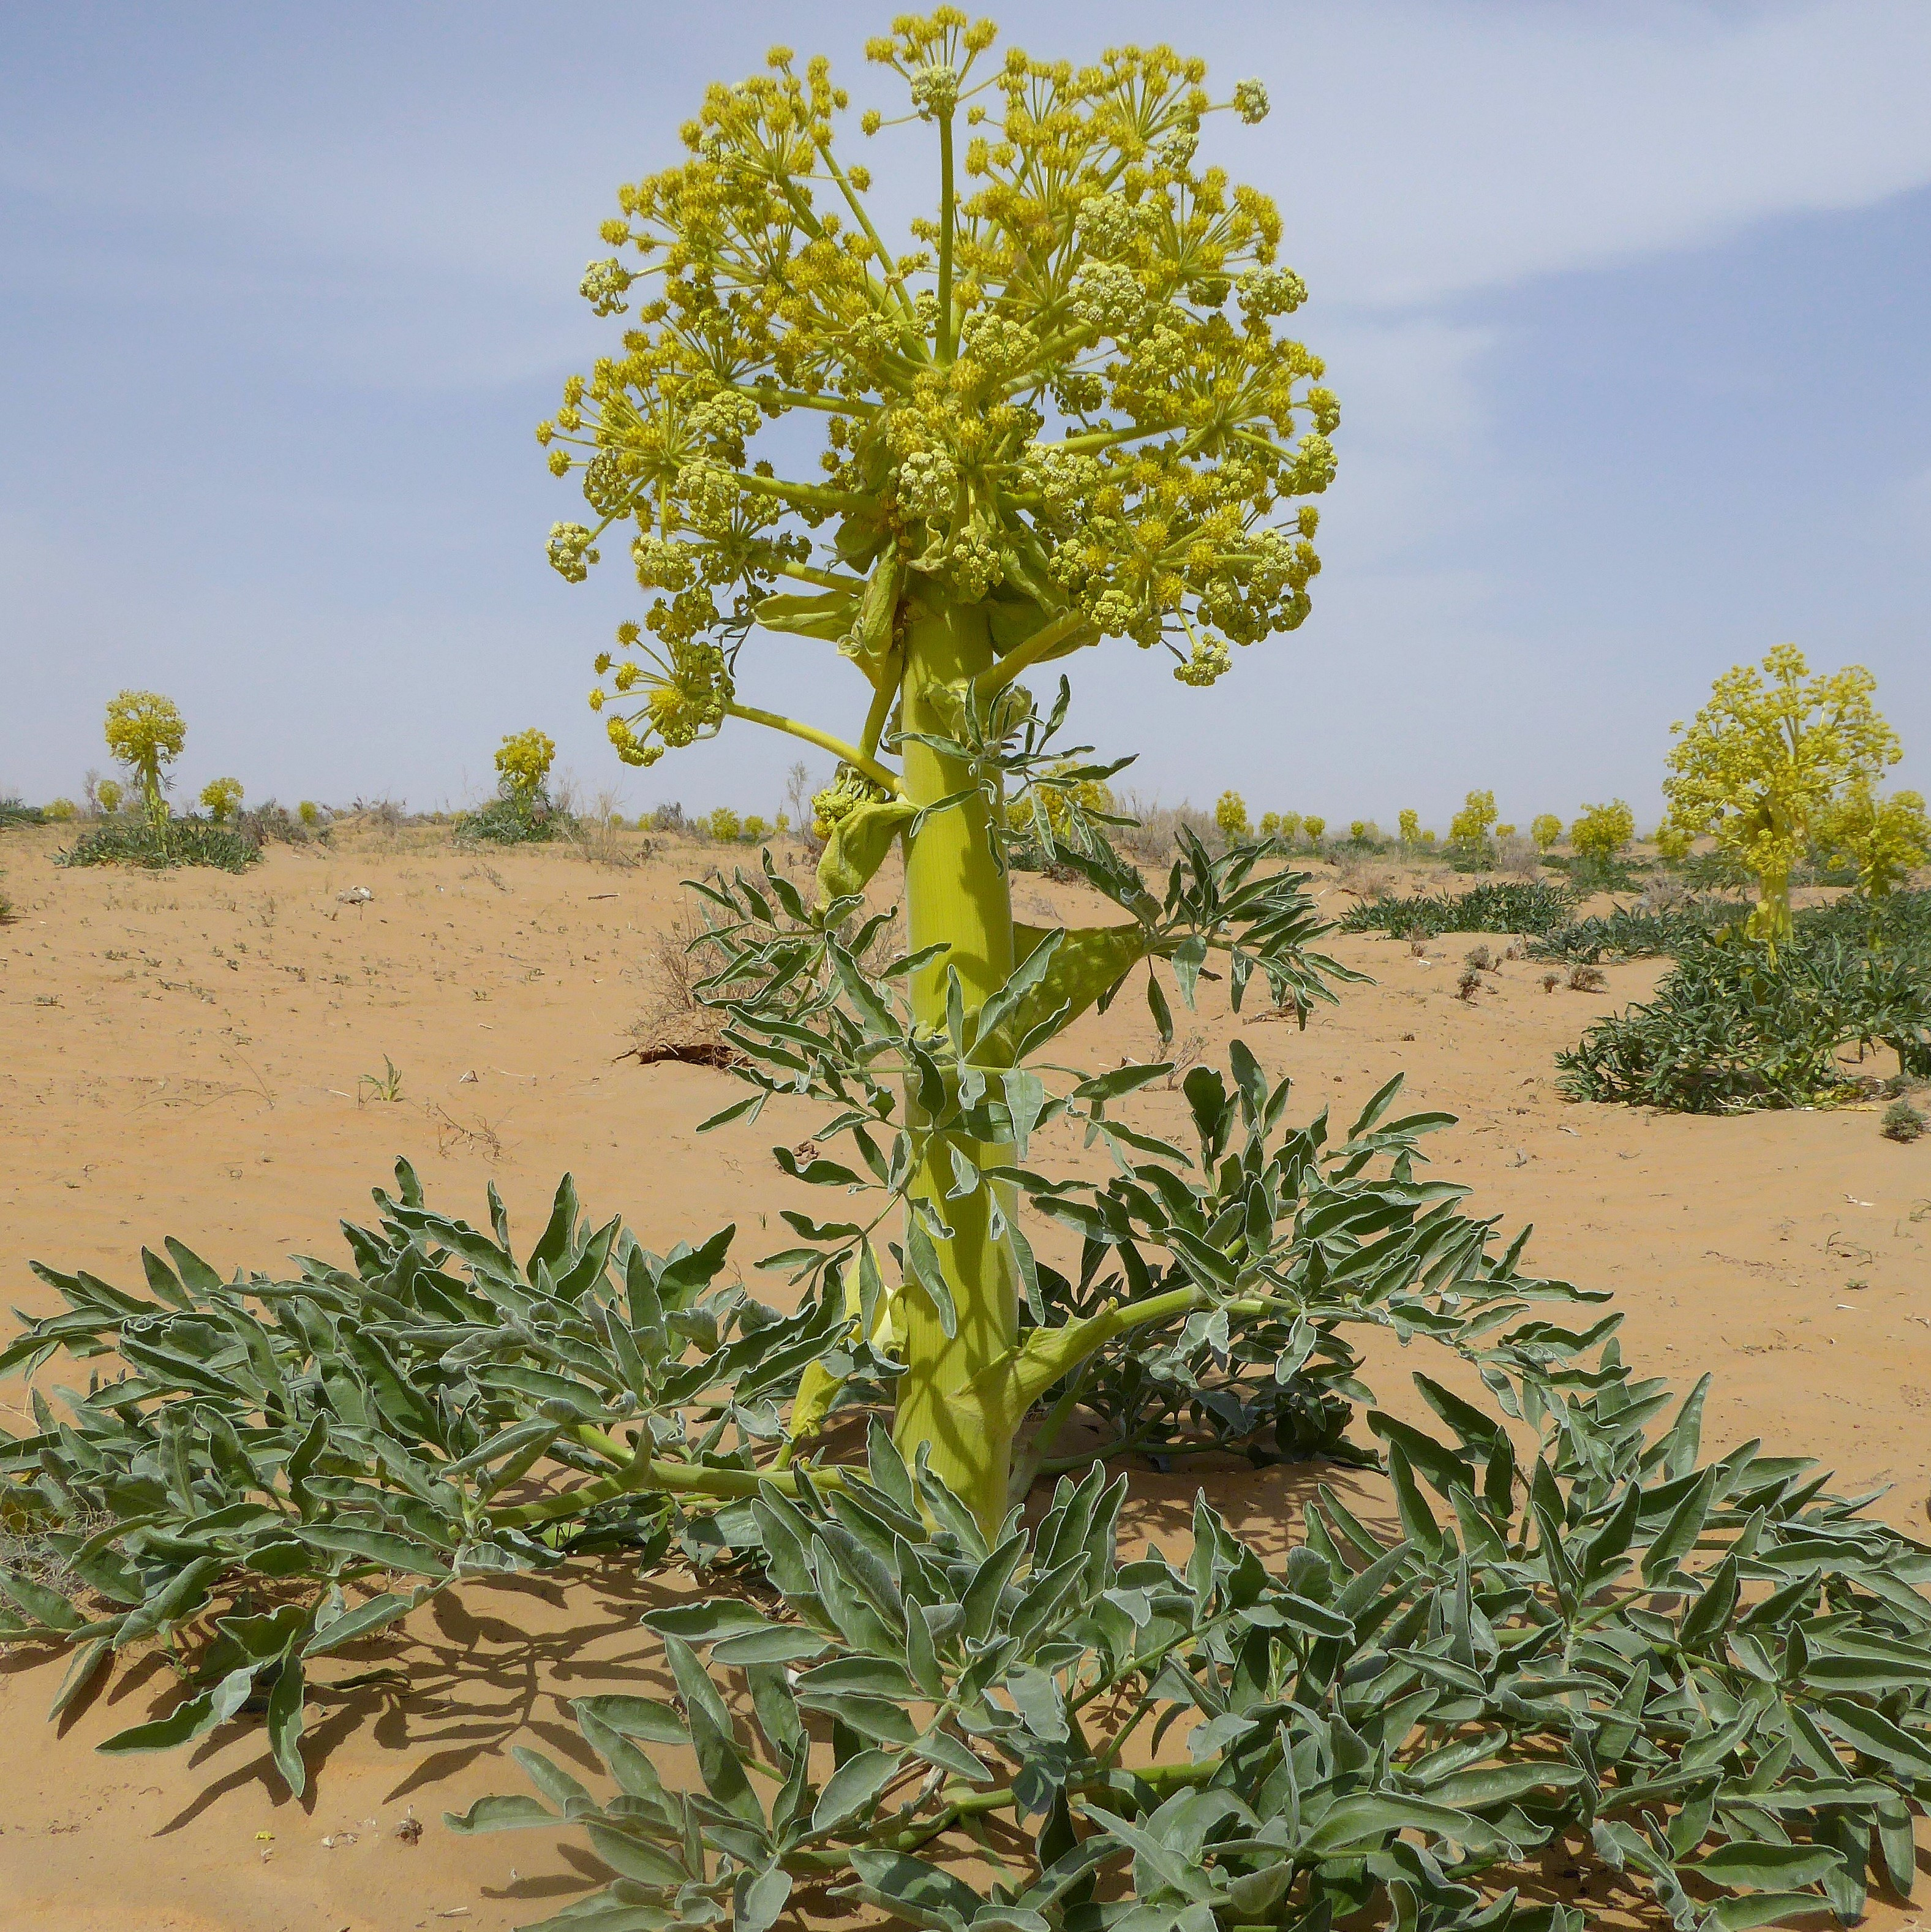
\includegraphics[width=0.3\linewidth]{imgs/spices/asafoetida-3.jpg}}
	\caption{Asafoetida in various forms, and one of its principal sources \taxon{Ferula assa-foetida} in the Kyzylkum Desert. Credit: Glorian; Aromatique; Public Domain.}
	\label{fig:asafoetida_imgs}
\end{figure}

Asafoetida is the dried, golden brown oleoresin that forms after cutting the stems of various ferula plants of Central Asia. The material itself is a waxy gum-resin, and it is sold either in gum or powdered form. Asafoetida is an extremely pungent, strong-smelling substance; it is described having a ``garlic-like'' and ``sulphurous odor'' that is sometimes too strong in itself and must be diluted with other materials \autocite[138]{van_wyk_culinary_2014}. Asafoetida is a drug and spice, and was used for centuries in both Asia and Europe \autocite{leung_itinerary_2019}. It is still an integral part of Indian cuisine as an ingredient, while in Europe and East Asia it was mainly utilized as medicine.

Regarding the characteristics and uses of the plant asafoetida, there are parallels with the now extinct giant ferula plant, which is believed to be the source of the lost silphium or laserpitium of antiquity. Silphium was a drug used in ointments of traditional Greek medicine, and a coveted ingredient in Roman cuisine. It was and introduced from Libya in North Africa, and was once a commercially crucial product featured on Roman coins. We now believe that over-harvesting led to its demise \autocites{dalby_dangerous_2000, leung_itinerary_2019, van_wyk_culinary_2014, langenheim_plant_2003}. 

\subsection{The Botany, Origin, and  Cultivation of Asafoetida}

%PLANT
Asafoetida is obtained from species of the genus \textit{Ferula} in the \textit{Apiaceae} family, such as \taxon{Ferula assa-foetida}, \taxon{F. foetida}, and \taxon{F. narthex} \autocite{mabberley_mabberleys_2017}. These plants are ``robust perennial herbs'' that can grow to 2 m high, and as umbelliferous plants surmounted by large yellow flowers \autocite[138]{van_wyk_culinary_2014}.
%ORIGIN
The plants cope well in mountainous and dry, desert-like conditions of Iran (from Yazd to Lar), up to Southern Uzbekistan (Kyzylkum Desert), and the Qandahar region of Afghanistan where they grow wild \autocite{leung_itinerary_2019}.
%CULT
Asafoetida is wild-harvested the same way it has been for thousands of years. The plant is cut before flowering, at the base of the stalk just above the root, and left exposed. The exudate is then collected once it solidifies, and this process is repeated again and again for up to three months, until no more liquid can be tapped \autocite[138]{van_wyk_culinary_2014}.

% culinary uses 
% Asafoetida is an important spice in Middle Eastern and South Asian cuisines and is widely used (especially in India) to flavour meat dishes, stews, gravies, sauces, mushrooms and pickles. When used sparingly, the offensive smell is lost during cooking, leaving a pleasant, garliclike aroma. The spice is not popular in Western cuisine but is (or was) allegedly an essential ingredient of Worcestershire sauce. 

% Used like onion or garlic.
% It was used by Jains and Brahmins because they do not eat onion! ??

% Flavour compounDs 
% The gum or oleoresin is a complex mixture of compounds, including ferulic acid esters, polysaccharide gums based on glucose, galactose and galacturonic acids, as well as terpenoids and coumarins.4,5 The odour is ascribed to various sulphides and sulfanes; secbutyl-propenyl disulphide (both E and Z isomers) are usually the main sulphur compounds.4,5 


% 1. Mabberley, D.J. 2008. Mabberley’s plant-book (3rd ed.). Cambridge University Press, Cambridge. 
% 2. Langenheim, J.H. 2003. Plant resins, pp. 412–417. Timber Press, Portland. 
% 3. Chamberlain, D.F. 1977. The identity of Ferula assa-foetida L. Notes from the Royal Botanic Garden, Edinburgh 35: 229–233. 
% 4. Rajanikanth, B., Ravindranath, B., Shankaranarayana, M.L. 1984. Volatile polysulphides of asafoetida. Phytochemistry 23: 899–900. 
% 5. Degenhardt, A. et al. 2012. Novel insights into the flavour chemistry of asafetida. In: Recent advances in the analysis of food and flavors, Chapter 12, pp. 167–175. American Chemical Society.

%  Teufelsdreck in German.

\subsection{The History of Asafoetida}

As ferula plants were not transplanted from Iran and Central Asia in the last couple thousands of years, its history and spread is connected with trade, especially overland.\footnote{According to news reports of last year, India, the biggest consumer of asafoetida only started experimenting with its cultivation in the last couple of years \autocite{express_news_service_taking_2021}.}   
A fantastic and recent chapter on the history of asafoetida already exists under the title \textit{The Itinerary of Hing/Awei/Asafetida
across Eurasia, 400–1800} by \textcite{leung_itinerary_2019}.

\subsection{The Names of Asafoetida}

\subsubsection{English}

\begin{etymology}\label{ety:asafoetida}
\textbf{English} \textit{asafoetida}, a. 1398
< \textbf{Medieval Latin} \textit{asafoetida} [stinking asa]
<\textss{?} from \textbf{Persian} \textit{āzā} `mastic', in a Lanized form, \textit{asa}
 + \textbf{Latin} \textit{foetid} `ill-smelling, stinking', (feminine of \textit{fœtidus})\footnote{\textcite[s.v. asafoetida]{oed}; \textcite[353]{laufer_sino-iranica_1919}; \textcite[42]{steingass_comprehensive_1892}}
\end{etymology}

\textit{Asafoetida} (also spelled \textit{asafetida}) is a term directly from Medieval Latin that found its way into the English lexicon via the early modern European medicinal and botanical literature. Often seen with archaic spellings, such as \textit{``assafœtida''}, the name is made up of the Latinized version of Persian \fa{ازا} \textit{aza/āzā}\footcite[][p. 42, \url{https://dsal.uchicago.edu/cgi-bin/app/steingass_query.py?page=42}]{steingass_comprehensive_1892} `mastic'\footnote{Mastic, also known as \textit{tears of Chios} is, a resin exuded from the trees \taxon{Pistacia lentiscus}. The dried, yellowish and translucent brittle pieces of resin resemble teardrops, and turn white when chewed, behaving like nature's (initially bitter) chewing gum. It is traditionally produced on the island of Chios, Greece.}, and Latin \textit{foetida}, feminine of \textit{foetidus} `stinking, ill-smelling, fetid' \footcite[asafoetida]{oed}. 

The first detailed discussion about asafoetida's name comes from \autocite[353-362]{laufer_sino-iranica_1919}'s \textit{Sino-Iranica}, where he vehemently opposes the theories of Persian origin regarding \textit{aza}, stating that its purported meaning, `mastic' is ``a product entirely different from what we understand by asafoetida'', and prefers the inferred theory first proposed by \textcite[41]{garcia_da_orta_colloquies_1913} that \textit{asa}---``mutilated by the druggists of the middle ages''---somehow derives from the \textit{laser} or Pliny's \textit{laserpitium} (a synonym for silphium, an important spice, medicine, and aphrodisiac used in antiquity just mentioned above). None of the two explanations are supported with documentary evidence, and he is right in that ``in no oriental language is there a word of the type asa or aza [...]''. I am not sure why did Laufer immediately dismiss the connection between mastic and asafoetida; both are obtained from the dried oleo-resin of Western and Central Asian plants, and even his own descriptions of mastic and its uses are very similar to that of asafoetida \autocite[252]{laufer_sino-iranica_1919}. His reports from a 1610 Chinese source, using the transcribed Arabic name \textit{mastaki} say that it is produced in Turkestan, used ``as \textit{jiao}'' (Sichuan pepper), and that its odor is very strong, and beneficial for digestion. Laufer, an expert in East Asian languages expects \textit{aza} to come up in other oriental languages, but it seems to me that the problem of \textit{aza} starts with Latin and therefore should be searched within the medieval European scientific literature. If \textit{aza}, a Persian term for a dried resinous substance (i.e. mastic) loaned by scribes of Latin existed, why does \textit{asa foetida}, literally `stinking mastic' for a foul smelling dried resinous gum sound so impossible? In fact, one of the Arabic names for asafoetida literally translates to `the mastic of the giant ferula'; but here `mastic' is likely to simply mean `gum'.

Asafoetida was first attested in Middle English, indicating its arrival in Europe. Sometime before 1398, we can read: ``Some stynkynge þinges beþ ydoon in medicyne, as..brymston and asa fetida.'' \footcite[asafoetida]{oed}. This illustrious entrance of asafoetida immediately points out its stench, and to be paired here with brimstone---once a synonym for sulfur, now a term chiefly used in a Biblical context in the description of hell (cf. ``fire and brimstone'')---is an apt premonition for the nickname \textit{devil's dung}. It is also worth noting that in English, the word first referred to the material, with the plant producing asafoetida sense only secondary; this is understandable, because no European have seen the ferula plants until the \nth{17} century, and the origins of the drug were obscure.

\begin{etymology}\label{ety:hing}
\textbf{English} \textit{hing} `asafoetida', 1599
< \textbf{Hindi} {हींग} \textit{hīng} `asafoetida'
< \textbf{Sanskrit} {हिङ्गु} \textit{hiṅgu} `asafoetida'; cf. cognates Sogdian 'ynkw
< \textbf{Proto-Iranian} \textit{*aṅgu-ǰatu-} `resin-gum'; cf. Tokharian B, Khotanese\footnote{\textcite[s.v. hing]{oed}; \textcite[s.v. hing]{oed}; \textcite[87]{gharib_sogdian_1995}; \textcite[7]{adams_dictionary_2013}}
\end{etymology}

India was always a big importer and consumer of asafoetida, and also played a role in exporting it to other part of the world. Bombay served as the key port in the \nth{19} century, where the stinking gum would change hands (sometimes after a bit of manipulation and adulteration). Contrary to China and Europe, Indians also developed an affinity to use it in their cooking. Thus, when the British came in contact with asafoetida in India, they adopted the local name: \textit{hing} \footcite[see][p. 418, \link{https://dsal.uchicago.edu/cgi-bin/app/hobsonjobson_query.py?qs=HING&searchhws=yes}]{yule_hobson-jobson_1903}. \textit{Hing} comes from Hindi \hi{हींग} 
\textit{hīṅg}, through Sauraseni Prakrit \textit{hiṁgu} from Sanskrit \sa{हिङ्गु}
\textit{hiṅgu}\footcite[hing]{ahd}. The Sanskrit term is believed to have derived from an Iranian source reconstructed as Proto-Iranian \textit{*aṅgu-ǰatu-} where \textit{ǰatu-}\footnote{\gls{PIE} \textit{*gʷétu} `resin, gum'} is `gum' (Modern Persian \fa{ژد} \textit{zhad} `gum') and other derivates are Tocharian B \textit{ankwaṣ(ṭ)}, Khotanese \textit{a\d{m}gu\d{s}\d{d}ä}, and Sogdian \textit{*angužat} \autocites[7]{adams_dictionary_2013}[87]{gharib_sogdian_1995}[281]{turner_comparative_1962}, also various Classical Persian forms, both inherited, e.g. \fa{انگدان} \textit{angudān}, \fa{آنغوزه} \textit{ānghuzah} and borrowed, e.g. \fa{انگژد} \textit{angužad} from Parthian \autocite[438]{tremblay_irano-tocharica_2005}. 

In English, \textit{hing} is first attested in Hakluyt's \textit{Principle Navigations} (new ed.): ``One hundred and fourescore boates laden with Salt, Opium, Hinge, Lead, Carpets [etc.].''\footcite[\url{http://www.perseus.tufts.edu/hopper/searchresults?target=en&inContent=true&q=hinge&doc=Perseus\%3Atext\%3A1999.03.0070}]{hakluyt_principall_1589}, and soon identified as a substance identical to asafoetida, as an example from 1662 shows: ``The Hingh, which our Drugsters and Apothecaries call Assa fœtida, comes for the most part from Persia.''\footcite[hing, \url{https://www.oed.com/view/Entry/87092}]{oed} 

Among its many vernacular names in European languages, such as \textit{devil's dung} in English, there is often a hint to the devil, possibly due to the connection between the smell of sulfur and hell in the Biblical tradition (``fire and brimstone''). The name \textit{devil's dung} in its various glosses is popular among European languages (e.g. German \textit{Teufelsdreck} lit. `devil's filth', Finnish \textit{pirunpihka} lit. `devil's resin', or Turkish \textit{şeytanboku} lit. `Satan's shit', which shows the strong aversion this material induces in European people, and why it never gained popularity in cookery. Other vernacular names in English include \textit{devil's dung}, \textit{asant}, \textit{stinking gum} \autocite[cf.][]{george_asafoetida_2012}. On the far opposite, the phrase ``food of the gods'' on Wikipedia actually links to asafoetida, because in an Indian context asafoetida was and is a desirable ingredient. Garcia da Orta, a Portuguese Jewish herbalist and ethnobotanist pioneer who spent much time on Goa wrote in the \nth{16} century:

\begin{quote}
    ``Well, you must know that the thing most used throughout India, and in all parts of it, is that Assa-fetida, as well for medicine as in cookery. A great quantity is used, for every Gentio who is able to get the means of buying it will buy it to flavour his food.'' \autocite[44]{garcia_da_orta_colloquies_1913}
\end{quote}

But as a European, he also notes on the next page: ``The nastiest smell in the world for me is Assa-fetida''.

\begin{table}[!ht]
\centering
\begin{tabularx}{\textwidth}{@{}l>{\itshape \small}lL>{\small}l@{}}
\toprule
\textbf{\#} & \multicolumn{1}{l}{\textbf{Species}} & \multicolumn{1}{l}{\textbf{Name}} & \multicolumn{1}{l}{\textbf{Source}} \\
\midrule
1	& Ferula assa-foetida et al.	& devil's dung	& \textcite{van_wyk_culinary_2014} \\
2	& Ferula assa-foetida et al.	& hing	& \textcite{van_wyk_culinary_2014} \\
3	& Ferula assa-foetida et al.	& stinking gum	& \textcite{peter_handbook_2012} \\
\textbf{4}	& \textbf{Ferula spp.}	& \textbf{asafoetida}	& \textbf{\textcite{van_wyk_culinary_2014}} \\
\bottomrule
\end{tabularx}
\caption{Various names for asafoetida in English.}
\label{table:names_asafoetida_en}
\end{table}



\subsubsection{Arabic}

\begin{etymology}\label{ety:hiltit}
Arabic {حلتيت} \textit{ḥiltīt} `asafoetida resin'; cf. cognates Hebrew \he{חִלְתִּית} \textit{ḥiltiṯ}
< Aramaic {\he{חלתיתא}/\sy{ܚܠܬܝܬܐ}} \textit{ḥeltīṯā} `id.'\footnote{\textcite[140]{fraenkel_aramaischen_1886}; \textcites[36]{low_aramaeische_1881}[vol. 3, p. 452-455]{low_flora_1924}}
\end{etymology}

Arabic terms now make a difference between the material and the plant; asafoetida as a spice/medicine is called \ar{حلتیت}
\textit{ḥiltīt}, while the plant is called \ar{انجدان} \textit{anjudān}.
The word \textit{ḥiltīt} comes from Aramaic \sy{ܚܠܬܝܬܐ} \textit{ḥeltīṯā}, and also exists in a Hebrew cognate as \he{חִלְתִּית} \textit{ḥiltiṯ}
\autocites[140]{fraenkel_aramaischen_1886}[36]{low_aramaeische_1881}[Vol. 3, p. 452-455]{low_flora_1924}. It is first attested in Sibawayhi's (ca. 760--796, a Persian native) \textit{al-Kitab [The Book]}, which is the earliest work on Arabic grammar and linguistics. \textit{Ḥiltīt} appears in the first Arabic dictionary, the \gls{Ayn} compiled by \textcite{al-farahidi_kitab_786}, simply sending the reader to \textit{al-anjudhān} `asafoetida', which could mean that this word was more widely known than \textit{ḥiltīt} at the time. \textit{Anjudān} is first mentioned in its earlier form \ar{انجذان} 
\textit{anjudhān} in the \citetitle{al-farahidi_kitab_786}, which also tells us that the source (\textit{u\d{s}\={u}l}) of \textit{anjudān} is a plant called \textit{maḥrūt}, which also appears in the poetry of Imru' l-Qays, the most eloquent poet of pre-Islamic Arabia \footcite[see][819]{ibn_manzur_lisan_1979}. Arabic \textit{anjudān} is a loanword from Persian, likely borrowed before the \nth{6} century and it comes from the same Proto-Iranian \textit{*aṅgu-ǰatu-} as Sanskrit, and later English \textit{hing}.

\begin{etymology}\label{ety:anjudan}
Arabic {أنجدان} \textit{anjudān}
< Persian {انگدان} \textit{angudān}
< Proto-Iranian \textit{*aṅgu-ǰatu-} `resin-gum'; cf. Tokharian B, Khotanese\footnote{\textcite[79-80]{lane_arabic-english_1863}; \textcite[114, 106]{steingass_comprehensive_1892}; \textcite[7]{adams_dictionary_2013}}
\end{etymology}

\begin{table}[!ht]
\centering
\begin{tabularx}{\textwidth}{@{}l>{\itshape \small}lr>{\itshape}lL>{\small}l@{}}
\toprule
\textbf{\#} & \multicolumn{1}{l}{\textbf{Species}} & \multicolumn{1}{l}{\textbf{Name}} & \multicolumn{1}{l}{\textbf{Tr.}} & \multicolumn{1}{l}{\textbf{Gloss}} & \multicolumn{1}{l}{\textbf{Source}} \\
\midrule
1	& Ferula spp.	& أبو كبير	& abū kabīr	& big father	& \textcite{wehr_dictionary_1976} \\
2	& Ferula spp.	& أنجدان	& anjudān	& 	& \textcite{baalbaki_-mawrid_1995} \\
3	& Ferula spp.	& صمغ الأجذان	& samgh al-anjudān	& gum of anjudan	& \textcite{baalbaki_-mawrid_1995} \\
4	& Ferula spp.	& صمغ راتيناجي	& samgh rātīnājī	& rātīnājī gum	& \textcite{baalbaki_-mawrid_1995} \\
\textbf{5}	& \textbf{Ferula spp.}	& \textbf{حلتیت}	& \textbf{ḥiltīt}	& \textbf{}	& \textbf{\textcite{wehr_dictionary_1976}} \\
\bottomrule
\end{tabularx}
\caption{Various names for asafoetida in Arabic.}
\label{table:names_asafoetida_ar}
\end{table}



\subsubsection{Chinese}

\begin{etymology}\label{ety:awei}
\textbf{Mandarin Chinese} \tc{阿魏} \textit{āwèi} MC /ʔɑ ŋʉiH/ `asafoetida'
< \textbf{Tokharian B} \textit{ankwaṣ(ṭ)} `asafoetida'
< \textbf{Sogdian} \textit{*angužat} `asafoetida'
< \textbf{Proto-Iranian} \textit{*aṅgu-ǰatu-} `resin-gum'\footnote{\textcite{leung_itinerary_2019}; \textcite[353]{laufer_sino-iranica_1919}; \textcite[438]{tremblay_irano-tocharica_2005}}
\end{etymology}

As for Chinese, \zh{阿魏} \textit{awei} is the term that gained much prevalence in the \nth{7} century \autocite{leung_itinerary_2019}. It seems likely that it was Kuchean traders from around the Tarim basin who first brought asafoetida to Chang'an, the Tang capital on the eastern terminus of the Silk Road. The consensus now among both Sinologists and experts on the languages of the Silk Road is that \textit{awei} is a loan from Tocharian B \textit{ankwaṣ(ṭ)}, originating from the same Proto-Iranian etymon as two of the above Arabic and English examples \autocites[353]{laufer_sino-iranica_1919}[121]{baxter_old_2014}.

\begin{etymology}\label{ety:xingqu}
Mandarin Chinese {興蕖/興渠/興瞿} \textit{xīngqú} \textsc{mc} MC /hɨŋ ɡɨʌ/ `asafoetida', phonetic transcription
< Sanskrit {हिङ्गु} \textit{hiṅgu} `asafoetida'
< Proto-Iranian* \textit{*aṅgu-ǰatu-} `resin-gum'; cf. Tokharian B, Khotanese\footnote{\textcite{leung_itinerary_2019}; \textcite[353]{laufer_sino-iranica_1919}; \textcite[7]{adams_dictionary_2013}}
\end{etymology}

But, there was an earlier name for asafoetida in Chinese: \zh{興蕖/瞿/渠} \textit{xingqu}, doublet of \zh{形虞} \textit{xingyu}. These are direct transcriptions of the Sanskrit \textit{hiṅgu} we mentioned above, and were attested in \nth{5}-century Buddhist sutras \autocite{leung_itinerary_2019}. It is also worth mentioning that in this case, the Chinese monks most likely had no idea what exactly \textit{xingqu} is, just that it some plant resin, and as such, it exemplifies a rare case when the word precedes the thing it refers to. In the \gls{BCGM}, besides the names above, other synonyms can also be found. These are \zh{阿虞} \textit{ayü}, from the transcription of Persian \textit{anguza(d)}, and \zh{哈昔尼} \textit{haxini}, the transcription of Ghazni, a city in Afghanistan where asafoetida was exported from. In the \gls{TPGJ} (citing the \gls{YYZZ}, it is said that \textit{awei} comes from the country of \zh{伽闍那} \gls{MC} /gaʑana/, which is likely a rendering of Ghazna, a variant of Ghazni.\footnote{\gls{CTP}---\url{https://ctext.org/taiping-guangji/414/awei?searchu=\%E9\%98\%BF\%E9\%AD\%8F&searchmode=showall\#result}}

From all the names, the most successful was unquestionably \textit{awei}, it enjoyed popularity for centuries, and further propagated into Sinoxenic words of Japanese \jp{阿魏 あぎ} \textit{agi}, Korean \ko{阿魏 아위} \textit{awi}, and Vietnamese \textit{ngui} \autocites{leung_itinerary_2019}.

I highly recommend both \textcite[]{laufer_sino-iranica_1919}'s \citetitle{laufer_sino-iranica_1919}, and \textcite{leung_itinerary_2019}'s \citetitle{leung_itinerary_2019} for those who are interested in asafoetida's journey and it names.  

% Say something about Middle Chinese phonology and Zhengzhang, Baxter-Sagart?}

\begin{table}[!ht]
    \caption{Various names for asafoetida in Chinese.}
\centering
\begin{tabularx}{\textwidth}{@{}l>{\itshape \small}ll>{\itshape}lL>{\small}l@{}}
\toprule
\textbf{\#} & \multicolumn{1}{l}{\textbf{Species}} & \multicolumn{1}{l}{\textbf{Name}} & \multicolumn{1}{l}{\textbf{Tr.}} & \multicolumn{1}{l}{\textbf{Gloss}} & \multicolumn{1}{l}{\textbf{Source}} \\
\midrule
1	& Ferula spp.	& \tc{阿虞}	& ayü	& 	& \textcite{leung_itinerary_2019} \\
2	& Ferula spp.	& \tc{哈昔尼}	& hāxīní	& 	& \textcite{leung_itinerary_2019} \\
3	& Ferula spp.	& \tc{黑黎提提}	& hēilítí​tí	& 	& \textcite{rossabi_eurasian_2013} \\
4	& Ferula spp.	& \tc{形虞}	& xíngyú	& 	& \textcite{leung_itinerary_2019} \\
5	& Ferula spp.	& \tc{興蕖/興渠/興瞿}	& xīngqú	& 	& \textcite{leung_itinerary_2019} \\
\textbf{6}	& \textbf{Ferula spp.}	& \textbf{\tc{阿魏}}	& \textbf{āwèi}	& \textbf{}	& \textbf{\textcite{leung_itinerary_2019}} \\
\bottomrule
\end{tabularx}
\label{table:names_asafoetida_zh}
\end{table}



\subsubsection{Summary}

And so, what we see here is that all three languages under scrutiny---English, Arabic, and Chinese---have at least one word that goes back to the same Proto-Iranian etymon, from the geographic source of the material it signifies and from the native region of the plant it is harvested from. This is not a surprise, rather evidence showing that the words do follow the material, even with twists and turns, and that tracing their journey correlates with the trade routes thus marking the contact zones where information about the material was transmitted.

\begin{table}[!ht]
\centering
\begin{tabularx}{\textwidth}{@{}ll>{\itshape}lLl>{\small}l@{}}
\toprule
\textbf{\#} & \textbf{Language} & \multicolumn{1}{l}{\textbf{Term}} & \textbf{Gloss} & \textbf{Loan} & \multicolumn{1}{l}{\textbf{Source}} \\
\midrule
1	& English	& devil's dung	& 	& no	& \textcite{oed} \\
2	& English	& hing	& 	& yes	& \textcite{oed} \\
3	& English	& asafoetida	& 	& yes	& \textcite{oed} \\
\midrule
1	& Arabic	& abū kabīr	& big father	& no	& \textcite{wehr_dictionary_1976} \\
2	& Arabic	& anjudān	& 	& yes	& \textcite{baalbaki_-mawrid_1995} \\
3	& Arabic	& samgh al-anjudān	& gum of anjudan	& no	& \textcite{baalbaki_-mawrid_1995} \\
4	& Arabic	& samgh rātīnājī	& rātīnājī gum	& no	& \textcite{baalbaki_-mawrid_1995} \\
5	& Arabic	& ḥiltīt	& 	& yes	& \textcite{wehr_dictionary_1976} \\
\midrule
1	& Chinese	& āwèi	& 	& yes	& \textcite{mdbg} \\
\bottomrule
\end{tabularx}
\caption{Conventionalized names for asafoetida in English, Arabic, and Chinese, found in dictionaries.}
\label{table:names_asafoetida}
\end{table}



\begin{figure}[ht]
    \centering
    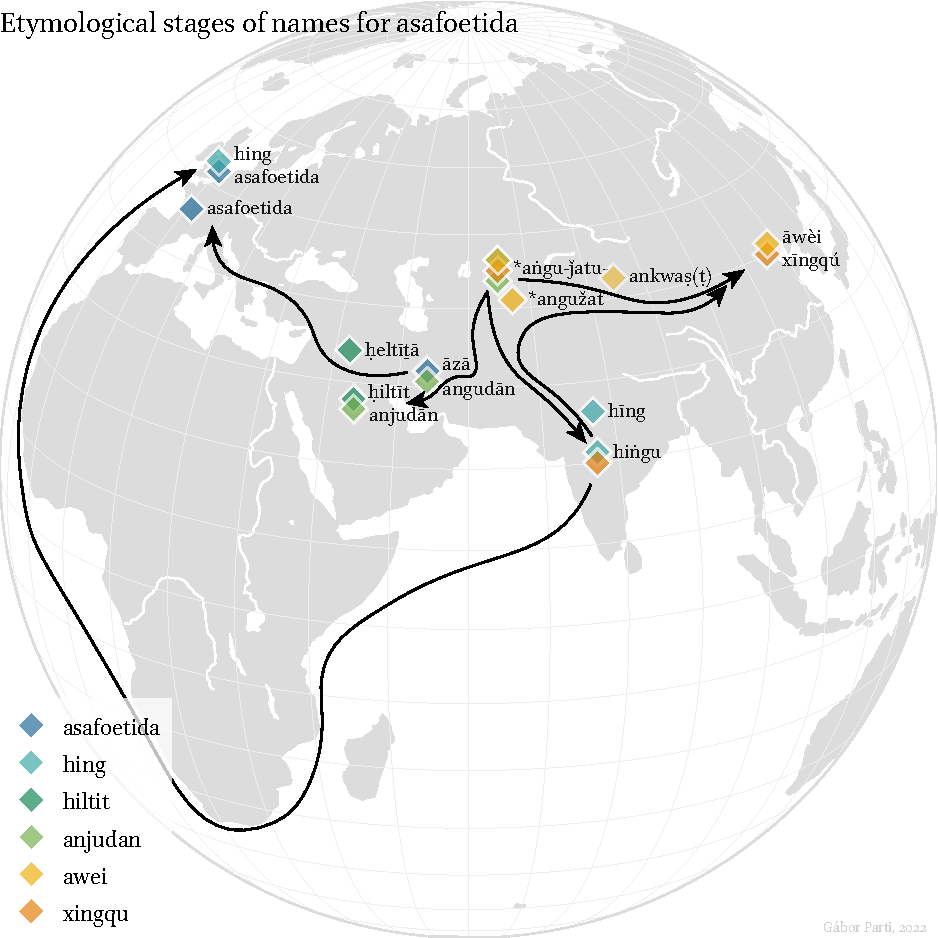
\includegraphics[width=\textwidth]{imgs/plots/diffusion_asafoetida_edited.pdf}
    \caption{Etymological stages in the progression of prototypical names of asafoetida.}
    \label{fig:cardamom_stages}
\end{figure}






% EE:
% asafoetida 
% resinous gum with a strong smell. XIV. — medL., lit. ‘stinking asa’, i.e. asa (usu. derived from a Persian azā mastic, but this word is of doubtful authenticity), fœtida, fem. of fœtidus FETID.

% OE:
% asafoetida (n.)
% alternative spelling of asafetida (q.v.); also see oe.
% asafetida (n.)
% "pungent sap from the roots of several plants native to Persia and Afghanistan," used as a drug, late 14c., from Medieval Latin asa (Latinized from Persian aza "mastic") + foetida, fem. of foetidus "stinking" (see fetid).

% MW:
% Middle English asafetida, from Medieval Latin asafoetida, from asa gum (of Iranian origin; akin to Persian azā mastic) + Latin foetida, feminine of foetidus fetid
% First Known Use: 14th century

% AH:
% [Middle English, from Medieval Latin asafētida : asa, gum (from Persian azā, mastic) + Latin foetida, feminine of foetidus, stinking; see FETID.]

% WK:
% Late Middle English, from Medieval Latin asafoetida, from Persian ازا / آزا (azâ, âzâ, “mastic”) + Latin foetida, feminine of foetidus (“bad-smelling”). 


% Synonyms: asant, hing, devil's dung

% MW:
% Hindi hī̃g, from Sanskrit hiṅgu

% AH:
% [Hindi, hīṁg, from Prakrit hiṁgu-, from Sanskrit hiṅgu, perhaps of Iranian origin; akin to Persian angu- in angužad, asafetida (angu- + žad, gum, tears of sap).]

% WK:
% From Hindi हींग (hīṅg). 




